\chapter{力制御}
油圧システムの力制御については,センサを取り付けて直接力を測定したり,\eqnname\ref{eq:fthr}による推力をそのままシリンダの出力として用いる方法がとられてきた\cite{semini2010design,semini2010hyq,川端健太郎20141a1,岡田大貴2017多自由度油圧駆動ロボットのシリンダ圧に基づく手先負荷力推定による力覚フィードバック}.
本章では,$\GfthrTofmsr$を用いて出力を推定する推定アルゴリズムおよび制御器の設計とその比較を行う.

\section{力推定アルゴリズム}
力制御をおこなうためのシステムのブロック線図を\figname\ref{fig:ForceEstimateControl}に示す.
油圧シリンダのhead側およびrod側の圧力と受圧面積から\eqnname\ref{eq:fthr}を用いて推力$\fthr$を計算して伝達関数$\GfthrTofmsr$へ入力し,その出力を推定出力$\fest$としてフィードバックする.
実際に発生している実測出力$\fmsr$はLoad Cellにより測定される.

\begin{figure}[t]
    \centering
%        \includegraphics[keepaspectratio, scale=1.0]{figurename.pdf}
        \begin{tikzpicture}
    [
        scale =1,
    % 線と文字の間の間隔を設定
    every node/.style={outer sep=0.12cm, inner sep=0},
    % 矢印の設定
    arrow/.style={-{Stealth[length=0.25cm]}, thick},
    % ブロック
    block/.style={rectangle, draw, minimum height = 1cm,
    minimum width=1.2cm, thick, outer sep = 0},
    block2/.style={rectangle, draw, minimum height = 2.5cm,
    minimum width=1.2cm, thick, outer sep = 0},
    % 加え合わせ点
    sum/.style={thick, circle, draw, inner sep=0,
    minimum size=6pt, outer sep=0},
    % 引き出し点
    point/.style={radius=2pt},
    %%
    gain/.style = {regular polygon, regular polygon sides=3,
        draw, fill=white, minimum width=1cm,
        inner sep=0, outer sep=0mm,
        shape border rotate=-90}
    ]
    \node [block] (K){~Controller~~};
    \node [block2, right=0.6 of K] (G){\begin{tabular}{l}Hydraulic\\Cylinder\end{tabular}};
    \node [sum, left=0.6of K] (sum){};    
    \coordinate (G1) at ($(G.north east)!0.25!(G.south east)$);
    \coordinate (G2) at ($(G.north east)!0.75!(G.south east)$);
    \node [gain, right=0.6of G1] (Ah){$\Ah$};
    \node [gain, right=0.6of G2] (Ar){$\Ar$};
    \node [sum,right=1.5 of G](sum2){};
    \node [block,right=-1cm of sum2,yshift = -2cm] (Gin2f){$\GinTofmsr$};
    

    \draw[arrow] (sum) -- (K);
    \draw[arrow] (K) -- (G) node [above, pos=0.5] {};
    \draw[arrow] (G1) -- (Ah) node[above,pos = 0.5]{$\phs$};
    \draw[arrow] (G2) -- (Ar) node[above,pos = 0.5]{$\prs$};
    \draw[arrow] (Ah) -| (sum2)node[left, yshift=+10pt] {$+$};
    \draw[arrow] (Ar) -| (sum2)node[right=0.3cm,yshift=0.3cm] {$\fthr$}
    node[left, yshift=-10pt] {$-$};
    \draw[arrow] (sum2) -|+(0.5,-1.3)-- +(-1.3,-1.3) |- (Gin2f);
    \draw[arrow] (Gin2f) -- +(2,0)node[right] {\begin{tabular}{l}Estimated\\Force\end{tabular}};
    \fill [point] (Gin2f)+(1.5, 0) circle coordinate (y);
    
    \draw[arrow] (G.north) |- +(2,1) node[right]{Measured Force};
    \draw[arrow] (sum.west)+(-0.5, 0) node[left]{\begin{tabular}{l}Set\\Point\end{tabular}} -- (sum.west)
    node[below, xshift=-10pt]{$+$};
    \draw [arrow] (y) -- +(0, -1) -| (sum) node[left, yshift=-15pt] {$-$};
\end{tikzpicture}
        \caption{Block Diagram for Force Control}
        \label{fig4:ForceEstimateControl}
\end{figure}


\section{PID制御とI-PD制御}
PID制御器(\figname\ref{fig4:PID})とI-PD制御器(\figname\ref{fig4:IPD})による応答を調べる.
I-PD制御器を利用するのは,目標値の急峻な変化に対するオーバーシュートを抑制させることを目的とするためである.
$s/(\tau s+1)$は近似微分器であり,$\tau=0.005$とした.
制御器におけるそれぞれのゲイン$K_P$,$K_I$,$K_D$は$\GinTofmsr$に対し限界感度法を適用して決定し,$K_P=8.4,~K_I =168,~K_D=0.1$とした.
\begin{figure}[t]
    \begin{minipage}{0.45\hsize}
    \centering
        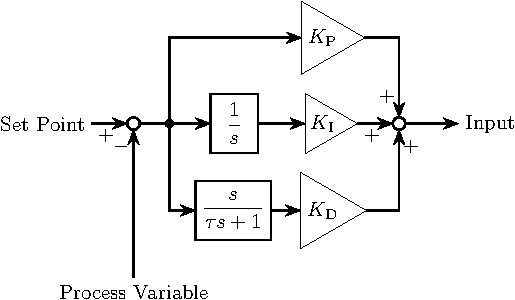
\includegraphics[keepaspectratio, width = \linewidth]{contents/ForceControl/figure/PIDcontroller-crop.pdf}
%        \begin{tikzpicture}
    [
        scale =1,
    % 線と文字の間の間隔を設定
    every node/.style={outer sep=0.12cm, inner sep=0},
    % 矢印の設定
    arrow/.style={-{Stealth[length=0.25cm]}, thick},
    % ブロック
    block/.style={rectangle, draw, minimum height = 1cm,
    minimum width=0.8cm, thick, outer sep = 0},
    block2/.style={rectangle, draw, minimum height = 2.5cm,
    minimum width=1.2cm, thick, outer sep = 0},
    % 加え合わせ点
    sum/.style={thick, circle, draw, inner sep=0,
    minimum size=6pt, outer sep=0},
    % 引き出し点
    point/.style={radius=2pt},
    %%
    gain/.style = {regular polygon, regular polygon sides=3,
        draw, fill=white, minimum width=0.8cm,
        inner sep=0, outer sep=0mm,
        shape border rotate=-90}
    ]
    \node [gain](KP){$K_\mathrm{P}$};
    \node [gain, below=0.7cm of KP] (KI){$K_\mathrm{I}$};
    \node [gain, below=0.7cm of KI](KD){$K_\mathrm{D}$};    
    \node [block,left=0.5cm of KD] (dev){~$\dfrac{s}{\tau s + 1}$~~};
    \node [block,left=0.8cm of KI] (int){$\dfrac{1}{s}$};
    \node [sum, right=0.6 of KI](sum){};
    \node[sum,left=1.2cm of int](u){};
    \node[left=0.6cm of u](SP){Set Point};
    \node[below=2.5cm of u](y){Process Variable};
    
    %\node[left=2cm of int](u){};



   \fill[point](int)+(-1.1,0) circle coordinate(u1);
   \draw[arrow](u1)|-(KP);
   \draw[arrow](KP)-|(sum)node[left=-0.05cm,yshift = 0.45cm]{$+$};
   \draw[arrow](u)--(int)node[above,pos=0.1]{};
   \draw[arrow](int)--(KI);
   \draw[arrow](KI)--(sum)node[left=0.2cm,yshift = -0.2cm]{$+$};
   \draw[arrow](u1)|-(dev);
   \draw[arrow](dev)--(KD);
   \draw[arrow](KD)-|(sum)node[right=-0.05cm,yshift = -0.4cm]{$+$};
   \draw[arrow](sum)-- +(1,0)node[right]{Input};
   \draw[arrow](SP) -- (u)node[left=0.2cm,yshift = -0.2cm]{$+$};
   \draw[arrow](y)--(u)node[left=-0.05cm,yshift = -0.4cm]{$-$};
%    \node [block] (K){~Controller~~};
%    \node [block2, right=0.6 of K] (G){\begin{tabular}{l}Hydraulic\\Cylinder\end{tabular}};
%    \node [sum, left=0.6of K] (sum){};    
%    \coordinate (G1) at ($(G.north east)!0.25!(G.south east)$);
%    \coordinate (G2) at ($(G.north east)!0.75!(G.south east)$);
%    \node [gain, right=0.6of G1] (Ah){$\Ah$};
%    \node [gain, right=0.6of G2] (Ar){$\Ar$};
%    \node [sum,right=1.5 of G](sum2){};
%    \node [block,right=-1cm of sum2,yshift = -2cm] (Gin2f){$\GinTofmsr$};
%    
%    
%    \draw[arrow] (sum) -- (K);
%    \draw[arrow] (K) -- (G) node [above, pos=0.5] {};
%    \draw[arrow] (G1) -- (Ah) node[above,pos = 0.5]{$\phs$};
%    \draw[arrow] (G2) -- (Ar) node[above,pos = 0.5]{$\prs$};
%    \draw[arrow] (Ah) -| (sum2)node[left, yshift=+10pt] {$+$};
%    \draw[arrow] (Ar) -| (sum2)node[right=0.3cm,yshift=0.3cm] {$\fthr$}
%    node[left, yshift=-10pt] {$-$};
%    \draw[arrow] (sum2) -|+(0.5,-1.3)-- +(-1.3,-1.3) |- (Gin2f);
%    \draw[arrow] (Gin2f) -- +(2,0)node[right] {\begin{tabular}{l}Estimated\\Force\end{tabular}};
%    \fill [point] (Gin2f)+(1.5, 0) circle coordinate (y);
%    
%    \draw[arrow] (G.north) |- +(2,1) node[right]{Measured Force};
%    \draw[arrow] (sum.west)+(-0.5, 0) node[left]{\begin{tabular}{l}Set\\Point\end{tabular}} -- (sum.west)
%    node[below, xshift=-10pt]{$+$};
%    \draw [arrow] (y) -- +(0, -1) -| (sum) node[left, yshift=-15pt] {$-$};

\end{tikzpicture}
        \subcaption{PID Controller}
        \label{fig4:PID}
    \end{minipage}
    \begin{minipage}{0.45\hsize}
    \centering
        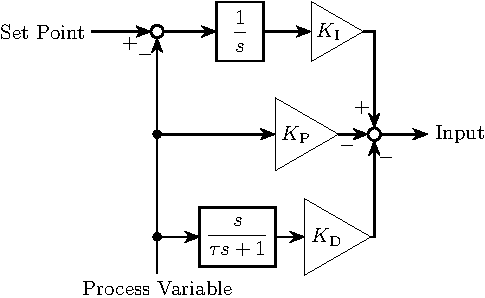
\includegraphics[keepaspectratio, width = \linewidth]{contents/ForceControl/figure/I-PDcontroller-crop.pdf}
%        \begin{tikzpicture}
    [
        scale =1,
    % 線と文字の間の間隔を設定
    every node/.style={outer sep=0.12cm, inner sep=0},
    % 矢印の設定
    arrow/.style={-{Stealth[length=0.25cm]}, thick},
    % ブロック
    block/.style={rectangle, draw, minimum height = 1cm,
    minimum width=0.8cm, thick, outer sep = 0},
    block2/.style={rectangle, draw, minimum height = 2.5cm,
    minimum width=1.2cm, thick, outer sep = 0},
    % 加え合わせ点
    sum/.style={thick, circle, draw, inner sep=0,
    minimum size=6pt, outer sep=0},
    % 引き出し点
    point/.style={radius=2pt},
    %%
    gain/.style = {regular polygon, regular polygon sides=3,
        draw, fill=white, minimum width=0.8cm,
        inner sep=0, outer sep=0mm,
        shape border rotate=-90}
    ]
    \node [sum](sum1){};
    \node [gain, right = 2.5cm of sum1] (KI){$K_\mathrm{I}$};
    \node [block,left=0.8cm of KI] (int){$\dfrac{1}{s}$};

    \node[below=3.6cm of sum1](y){y};
    \node[left=1cm of sum1](r){Set Point};
       
    \coordinate (y1) at ($(sum1)!0.4!(y)$);
    \coordinate (y2) at ($(sum1)!0.8!(y)$);
    \node [gain, right=2cm of y1] (KP){$K_\mathrm{P}$};
    \node [gain, right=2.5cm of y2](KD){$K_\mathrm{D}$};    
    \node [block,left=0.5cm of KD] (dev){~$\dfrac{s}{\tau s + 1}$~~};

    \node [sum,right=0.5cm of KP](sum2){};
    \node[right=0.8cm of sum2](input){Input};
    
    \fill[point](y1) circle coordinate;
    \fill[point](y2) circle coordinate;
    
    \draw[arrow](y)--(sum1)node[left=-0.05cm,yshift = -0.4cm]{$-$};
    \draw[arrow](r)--(sum1)node[left=0.2cm,yshift = -0.2cm]{$+$};
    \draw[arrow](sum1)--(int);
    \draw[arrow](int)--(KI);
    \draw[arrow](KI)-|(sum2)node[left=-0.05cm,yshift = 0.45cm]{$+$};
    \draw[arrow](y1)--(KP);
    \draw[arrow](KP)--(sum2)node[left=0.2cm,yshift = -0.2cm]{$-$};
    \draw[arrow](y2)--(dev);
    \draw[arrow](dev)--(KD);
    \draw[arrow](KD)-|(sum2)node[right=-0.05cm,yshift = -0.4cm]{$-$};
    \draw[arrow](sum2)--(input);
    
    
    
%    \fill[point](int)+(-1.2,0) circle coordinate(u1);
%    \draw[arrow](u1)|-(KP);
%    \draw[arrow](KP)-|(sum)node[left=-0.05cm,yshift = 0.45cm]{$+$};
%    \draw[arrow](u)--(int)node[above,pos=0.1]{error};
%    \draw[arrow](int)--(KI);
%    \draw[arrow](KI)--(sum)node[left=0.2cm,yshift = -0.2cm]{$+$};
%    \draw[arrow](u1)|-(dev);
%    \draw[arrow](dev)--(KD);
%    \draw[arrow](KD)-|(sum)node[right=-0.05cm,yshift = -0.4cm]{$+$};
%    \draw[arrow](sum)-- +(1,0)node[above]{input};


%    \node [block] (K){~Controller~~};
%    \node [block2, right=0.6 of K] (G){\begin{tabular}{l}Hydraulic\\Cylinder\end{tabular}};
%    \node [sum, left=0.6of K] (sum){};    
%    \coordinate (G1) at ($(G.north east)!0.25!(G.south east)$);
%    \coordinate (G2) at ($(G.north east)!0.75!(G.south east)$);
%    \node [gain, right=0.6of G1] (Ah){$\Ah$};
%    \node [gain, right=0.6of G2] (Ar){$\Ar$};
%    \node [sum,right=1.5 of G](sum2){};
%    \node [block,right=-1cm of sum2,yshift = -2cm] (Gin2f){$\GinTofmsr$};
%    
%    
%    \draw[arrow] (sum) -- (K);
%    \draw[arrow] (K) -- (G) node [above, pos=0.5] {};
%    \draw[arrow] (G1) -- (Ah) node[above,pos = 0.5]{$\phs$};
%    \draw[arrow] (G2) -- (Ar) node[above,pos = 0.5]{$\prs$};
%    \draw[arrow] (Ah) -| (sum2)node[left, yshift=+10pt] {$+$};
%    \draw[arrow] (Ar) -| (sum2)node[right=0.3cm,yshift=0.3cm] {$\fthr$}
%    node[left, yshift=-10pt] {$-$};
%    \draw[arrow] (sum2) -|+(0.5,-1.3)-- +(-1.3,-1.3) |- (Gin2f);
%    \draw[arrow] (Gin2f) -- +(2,0)node[right] {\begin{tabular}{l}Estimated\\Force\end{tabular}};
%    \fill [point] (Gin2f)+(1.5, 0) circle coordinate (y);
%    
%    \draw[arrow] (G.north) |- +(2,1) node[right]{Measured Force};
%    \draw[arrow] (sum.west)+(-0.5, 0) node[left]{\begin{tabular}{l}Set\\Point\end{tabular}} -- (sum.west)
%    node[below, xshift=-10pt]{$+$};
%    \draw [arrow] (y) -- +(0, -1) -| (sum) node[left, yshift=-15pt] {$-$};

\end{tikzpicture}
        \subcaption{I-PD Controller}
        \label{fig4:IPD}
    \end{minipage}
    \caption{PID and I-PD Controller}
\end{figure}

それぞれの制御器におけるステップ応答を\figname\ref{fig4:SRofPIDandIPD}に示す.
\figname\ref{fig4:SR_fest}が推定値の応答,\figname\ref{fig4:SR_fmsr}が実測出力の応答である.
\figname\ref{fig4:SR_fest}より推定値$\fest$は目標値に対し定常偏差なく追従している.
実測出力$\fmsr$の応答は,\figname\ref{fig4:SR_fmsr}より定常偏差が残っていることが確認されるが,偏差は\SI{5}{\%}以内に収まっており,推定値をフィードバックすることにより実測出力を制御することができているといえる.
また,I-PD制御器におけるオーバーシュートがPID制御器に比べて抑制されており,I-PD制御器を導入した意図を満たしている.

\begin{figure}[tbp]
    \begin{minipage}{0.45\hsize}
        \centering
        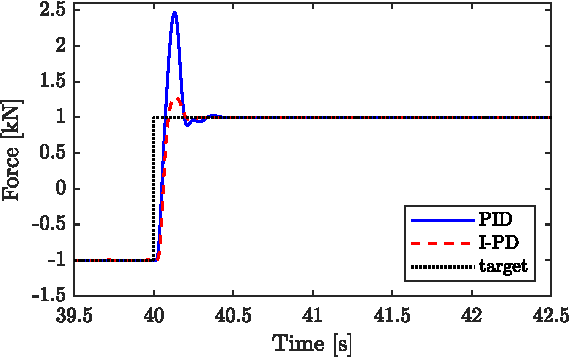
\includegraphics[keepaspectratio, width = \linewidth]{contents/ForceControl/figure/1115_PIDandI-PDestforce_step.pdf}
        \subcaption{Estimated Force:$\fest$}
        \label{fig4:SR_fest}
    \end{minipage}
    \begin{minipage}{0.45\hsize}
        \centering
        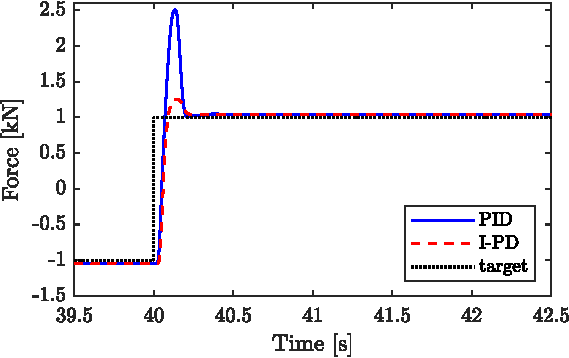
\includegraphics[keepaspectratio, width = \linewidth]{contents/ForceControl/figure/1115_PIDandI-PDforce_step.pdf}
        \subcaption{Measured Force:$\fmsr$}
        \label{fig4:SR_fmsr}
    \end{minipage}
    \caption{Step Repsonse of PID Controller and I-PD Controller}
    \label{fig4:SRofPIDandIPD}
\end{figure}


\section{$H_\infty$制御}
対象のシステムに対して,$H_\infty$制御の適用をする.
$H_\infty$制御の適用により,モデル化誤差の吸収および外乱抑制が期待される.
力制御を行う際には環境との接触を伴うため,環境から振動など様々な外乱を受けることになる.
その点においても,外乱抑制を行う制御の適用は意味あるものとなる.
\subsection{対象システムの状態空間表現}

\subsection{$H_\infty$制御器}
\subsection{サーボ系$H_\infty$制御器}

\section{外乱に対する頑健性}

